\documentclass[11pt,a4paper]{article}
\usepackage[author={Lyndon}]{pdfcomment}

\usepackage{booktabs}
\usepackage{pgfplotstable}
\pgfplotsset{compat=1.14}

\usepackage{url}


\usepackage{tikz}
\usetikzlibrary{positioning, fit,  shapes.geometric}
\tikzset{
	node distance=1cm and 1.5cm,
	every text node part/.style= {
		align=center
	},
	word/.style= {
		blue,
		font=\itshape,
	},
	layer/.style= {
		rectangle, 
		black,
		draw
	}
}


\usepackage{graphicx}
\graphicspath{{./figs/}, {./}}


\usepackage[subpreambles=false]{standalone}

\usepackage{amssymb}
\usepackage{amsmath}
\usepackage{mathtools}
\DeclareMathOperator*{\argmin}{arg\,min}
\DeclareMathOperator*{\argmax}{arg\,max}




\usepackage{cleveref}

%%%%%%%%%%%%%%%%%%%%%%%%%%%%%%%%%%%%
\usepackage{url}
\usepackage{natbib}


\newcommand{\parencite}{\citep}
\newcommand{\textcite}{\citet}


%%%%%%%%%%%%%


\newcommand{\natlang}[1]{\texttt{#1}}
%%%%%%%%%%%%%%%%%%%%%%%%%%%%%%%%%%%%%%
%opening
\title{Estimating Intended Color from its Name}
\author{Lyndon White, %
	Roberto Togneri, %
	Wei Liu, %
	\and Mohammed Bennamoun%
	\\ 
	\url{lyndon.white@research.uwa.edu.au}, %
	\url{roberto.togneri@uwa.edu.au},\\
	\url{wei.liu@uwa.edu.au}, %
	\and \url{mohammed.bennamoun@uwa.edu.au}%
	\\
	The University of Western Australia.
	35 Stirling Highway, Crawley, Western Australia
}



\begin{document}

\maketitle

\begin{abstract}
When a speaker says the name of a color, the color that they picture is not necessarily the same as the listener imagines.
Color is a grounded semantic task, but that grounding is not a mapping of a single word or phrase to a single point in color-space.
Proper understanding of color language requires the capacity to map a sequence of words to a probability distribution in color-space.
A distribution is required as there is no clear agreement between people as to what a particular color describes -- different people have a different idea of what it means to be ``very dark orange''.

Learning how each word in a color name contributes to the color described,
allows for knowledge sharing between uses of the words in different color names.
This knowledge sharing significantly improves predicative capacity for color names with sparse training data.
The extreme case of this challenge in data sparsity is for color names without any direct training data.
Our model is able to predict reasonable distributions for these cases, as evaluated on a held-out dataset consisting only of such terms.
\end{abstract}

\section{Introduction}\label{sec:intro}

Color understanding is an important subtask in natural language understanding.
It is a challenging domain, due to ambiguity, multiple roles taken by the same words, the many modifiers, and shades of meaning.
Due to its difficulty, texts containing color descriptions such as \texttt{the flower has petals that are bright pinkish purple with white stigma} are used as demonstrations for state of the art image generation systems \parencite{reed2016generative, 2015arXiv151102793M}.
The core focus of the work we present here is addressing these linguistic phenomena around the descriptions of the color, in a single patch, as represented in a color-space such as HSV \parencite{smith1978color}.
Issues of illumination and perceived color based on visual context are considered out of the scope.




\section{Related Work}\label{sec:related-work}
The understanding of color names has long been a concern of psycholinguistics and anthropology  \parencite{berlin1969basic,heider1972universals,HEIDER1972337,mylonas2015use}.
It is thus no surprise that there should be a corresponds field of research in natural language processing.

The earliest works revolve around explicit color dictionaries.
This includes the ISCC-NBS color system \parencite{kelly1955iscc} of 26 words, including modifiers, that are composed according to a context free grammar such that phrases are mapped to single points in the color-space;
and the simpler, non-compositional, 11 basic colors of \textcite{berlin1969basic}.
Works including \textcite{Berk:1982:HFS:358589.358606,conway1992experimental,ele1994computational, mojsilovic2005computational, menegaz2007discrete,van2009learning} which propose methods for the automatic mapping of colors to and from these small manually defined sets of colors.
We note that \textcite{menegaz2007discrete,van2009learning} both propose systems that discretize the color-space, though to a much courser level than we consider in this work.


More recent works, including the work presented here, function with much larger number of colors, larger vocabularies, and larger pools of respondents.
In particular making uses of the large Munroe dataset \textcite{Munroe2010XKCDdataset}, as we do here.
This allows a data driven approach towards the modelling.

\textcite{mcmahan2015bayesian} and \textcite{meomcmahanstone:color} present color naming methods, mapping from colors to to their names, the reverse of our task.
These works are based on defining fuzzy rectangular distributions in the color-space to cover the distribution estimated from the data, which are used in a Bayesian system to non-compositionally determine the color name.
%
%\pdfcomment{During the similar time-period another online color naming survey was conducted.
%\textcite{mylonas2010online,mylonas2012colour} collected a total of 50,000 observations from 2500 respondents in 7 languages.
%In this work we use the larger, more publically available, Munroe dataset.}
%
\textcite{2016arXiv160603821M} maps a point in the color-space, to a sequence of probability estimates over color terms.
They extends beyond, all prior color naming systems to produce a compositional color namer based on the Munroe dataset.
Their method uses a recurrent neural network (RNN), which takes as input a color-space point, and the previous output word, and gives a probability of the next word to be output -- this is a conditional language model.
In this work we tackle the inverse problem to the creation of a conditional language model.
Our distribution estimation models map from a sequence of terms, to distribution in color space.
Similarly, our point estimation models map from sequence of terms to single point in color-space.



\textcite{DBLP:journals/corr/KawakamiDRS16} propose another compositional color naming model.
They use a per-character RNN and a variational autoencoder approach.
It is in principle very similar to \textcite{2016arXiv160603821M}, but functioning on a character, rather than a word level.
The work by Kawakami et al. also includes a method for generating colors.
However they only consider the generation of point estimated, rather than distributions.
The primary focus of our work is on generating distributions.
The datasets used by Kawakami et al. contain only very small numbers of observations for each color name (often just one).
These datasetsare thus not suitable for modelling the distribution in color space as interpreted by the population.
Further, given the very small number of examples they are not well suited for use with word-based modelling: the character based modelling employed by Kawakami et al. is much more suitable.
As such we do not attempt comparison to their work.


\textcite{DBLP:journals/corr/MonroeHGP17} presents a neural network solution to a communication game, where a speaker is presented with three colors and asked to describe one of them, and the listener is to work out which is being described.
Speaker and listener models are trained, using LSTM-based decoders and encoders respectively.
The final time-step of their model produces a 100 dimensional representation of the description provided.
From this, a Gaussian distributed score function is calculated, over a high dimensional color-space from \textcite{2016arXiv160603821M}, which is then used to score each of the three options.
While this method does work with a probability distribution, as a step in its goal,
this distribution is always both symmetric and unimodal -- albeit in a high-dimensional color-space.

The generation of color from text has not received a signficant ammount of attention in prior work.
In particular the generation of probability distributions in color space, to our knowledge has not been considered at all.
Conversely, there has been several works on the reverse problem: the generation of a textual name for a color from color space point.
The work presented here closed that gap.

Consider that the word \texttt{tan} may mean one of many colors for different people in different circumstances: ranging from the bronze of a tanned sunbather, to the brown of tanned leather;
\texttt{green} may mean anything from \texttt{aquamarine} to \texttt{forest green};
and even \texttt{forest green} may mean the rich shades of a rain-forest, or the near grey of the Australian bush.
Thus the color intended cannot be uniquely inferred from the color name.
Without further context, it does nevertheless remain possible to estimate likelihoods of which colors are be intended based on the population's use of the words.
The primary aim of this work is to map a sequence of color description words to a probability distribution over a color-space.
This is required for a proper understanding of color language.
We also consider the more basic point estimation of colors, though it's value is questionable.


Proper understanding requires considering \emph{the color intended} as a random variable.
In other words, a color name should map to a distribution, not just a single point or region.
For a given color name, any number of points in the color-space could be intended, with some being more or less likely than others.
Or equivalently, up to interpretation, it may intend a region but the likelihood of what points are covered is variable and uncertain.
This distribution is often multimodal and has high and asymmetrical variance, which further renders regression to a single point unsuitable.
We do produce results point estimate results for interest in \Cref{sec:results-point-est}, however for any form of precise work the use of such systems is limited
A single point estimate, does not capture the nature of the problem adequately.
The mean of a multimodal distribution (one with two peaks) will lie in the valley between the -- a less likely color.
Similarly it will be off to the side of the mode, in an asymmetrical distribution
Thus whi 


We estimate a probability distribution over the color-space.
To qualify our estimate of the distribution we discretize the space into a large number of patches, and produce an output much like a histogram.
This allows us to take advantage of the well-known softmax based methods for estimating a probability mass distribution using a neural network.


Estimating color probabilities has a clear use as a subsystem in many systems.
For example, in a human-interfacing system, when asked to select the \texttt{dark bluish green} object, each object can be ranked based on how likely its color is according to the distribution.
This way if extra information eliminates the most-likely object, the second most likely object can immediately be determined.
Further, if the probability of the color of the object being described by the user input is known, a threshold can be set to report that no object is found, or to ask for additional information.
More generally, the distribution based on the color name alone can be used as a prior probability and combined with additional context information to yield better predictions.







\section{Method}
\subsection{Tokenization}
For all the term based methods, we perform tokenization.
Tokenization 

\subsubsection{HSV color-space}
We use the HSV color-space \parencite{smith1978color}.
through-out this work.
We use the format which the data is originally provided in.
In this format hue, saturation and value all range between zero and one.
Unlike many other colors spaces (CIELab, Luv etc.) the gamut is square.
This regular space means that errors on all channels can be considered equally, and unlike other color spaces.
The scaling of hue in particular to be between zero and one (like the other channels) makes the modelling task more consistent as were the hue to range between $0$ and $2\pi$ it would be over-weighted compared to the other channels.

When working with the hue, all measures need to take into account the wrap-around effect.
When ever we refer to mean squared error, mean or mode on the HSV space in this paper, we are referring to the angularly corrected forms given in \Cref{sec:angularly-correct}.


Unlike the RGB color space, the HSV channels do correspond to how humans perceive colors.
However, it is not designed to be a perceptionally uniform color space across hue (unlike CIELab), which does suggest using mean squared error for the point estimates is not optimal.
However, given the other issues outlined above with point estimates we do not judge this a major concern.
There are no such issues for our distribution estimations.

One of it's important advantages over other color spaces is that it best meets the assumption that for a given color name each channel is statistically independent.

\subsection{Angularly Correct Calculations on HSV}\label{sec:angularly-correct}
When performing calculations with the HSV color space it is important to take into account that hue is an angle.
As we are working with the color space regularized to range between zero and one for all channels,
this means a hue of one and a hue of zero are equivalent (in radian's this would be $0$ and $2\pi$).

The square error of two hue values is thus calculated as
\begin{equation}
SE(h_1, h_2) = \min \big( \left(h_1 - h_2 \right)^2, \, \left(h_1 - h_2 -1 \right)^2  \big)
\end{equation}
(using radians the $-1$ would be $-2\pi$)
to take into account the error could be calculated clockwise or counter clockwise.


The mean of a series of  $N$ hue values is calculated as 
\begin{equation}
\bar h = \mathrm{atan2} \Bigg(%
	\frac{1}{N} \sum_{i=1}^{i=N} \sin (h_i), \,  %
	\frac{1}{N} \sum_{i=1}^{i=N} \cos (h_i)%
\Bigg)%
\end{equation}
As we are using the regularized angle, we use the regularized versions of the trigonometric functions (though this shift is no different from degrees to radians).




\section{Distribution Estimation}
\subsection{Conditional Independence Assumption}\label{sec:conditional-independence-assumption}
We make the assumption that given the name of the color, the distribution of the H, S and V channels are independent.
That is to say, it is assumed if the color name is known, then  knowing the value of one channel would not provide any additional information as to the value of the other two channels.
The same assumption is made, though not remarked upon, in \textcite{meomcmahanstone:color} and \textcite{mcmahan2015bayesian}.
This assumption of conditional independence allows considerable saving in computational resources.
Approximating the 3D joint distribution as the product of three 1D distributions decreases the space complexity from $O(n^3)$ to $O(n)$ in the discretized step that follows.

Superficial checks were carried out on the accuracy of this assumption.
Spearman's correlation on the training data suggests that for over three quarters of all color names, there is only weak correlation between the channels (\mbox{Q3 = 0.187}).
However, this measure underestimates correlation for values that have circular relative value, such as hue.
HSV had the lowest correlation by a large margin of the 16 color-spaces evaluated.
Full details, including the table of correlations, are available in supplementary materials.
These results are suggestive, rather than solidly indicative, on the degree of correctness of the conditional independence assumption.
We consider the assumption sufficient for this investigation.

\subsection{Discretization}
For distribution estimation, our models are trained to output histograms.
By making use of the conditional independence assumption \Cref{sec:conditional-independence-assumption}, we output one histogram per channel.


\subsection{Kernel-Density Based Smoothing}\label{sec:kernel-density-based-smoothing}


We make use of the \textcite{silverman1982algorithm}








\section{Experimental Setup}

\subsection{Implementation}
The implementation of the CDEST and baseline models was in the Julia programming language \parencite{Julia}.
The full implementation is included in the supplementary materials.
can be downloaded from the GitHub repository.\footnote{Implementation source is at \url{https://github.com/oxinabox/ColoringNames.jl}}
It makes heavy use of the MLDataUtils.jl\footnote{MLDataUtils.jl is available from \url{https://github.com/JuliaML/MLDataUtils.jl}} and TensorFlow.jl,\footnote{TensorFlow.jl is available from \url{https://github.com/malmaud/TensorFlow.jl}} packages.
the latter of which we enhanced significantly to allow for this work to be carried out.


\subsection{Common Network Features}
Dropout\parencite{srivastava2014dropout}  is used on all layers, other than the embedding layer, with threshold of 0.5 during training.
The network is optimized using Adam
\cite{kingma2014adam}, using a learning rate of 0.001.
Early stopping is checked every 10 epochs using the development dataset.
Distribution estimation methods are trained using full batch (where each observation is a distribution) for every epoch.
Point Estimation trains using randomized mini-batches of size $2^16$ observations (which are each color-space triples).
All hidden-layers, except as otherwise precluded (in side the convolution, and in the penultimate layer of the point estimation networks) have the same width 300, as does the the embedding layer.


\subsubsection{Embeddings}
All our neural network based solutions incorporate an embedding layer.
This embedding layer maps from tokenized words to vectors.
We make use of 300d pretrained FastText embeddings \textcite{bojanowski2016enriching}\footnote{Available from \url{https://fasttext.cc/docs/en/english-vectors.html}}.

The embeddings are not trained during the task, but are kept fixed.
As per the universal approximation theorem \parencite{leshno1993uat, SONODA2017uat} the layers above allow for arbitrary non-linear continuous transformation.




\subsection{Input Modules}


\subsubsection{Recurrent Neural Network(RNN)}
\begin{figure}
	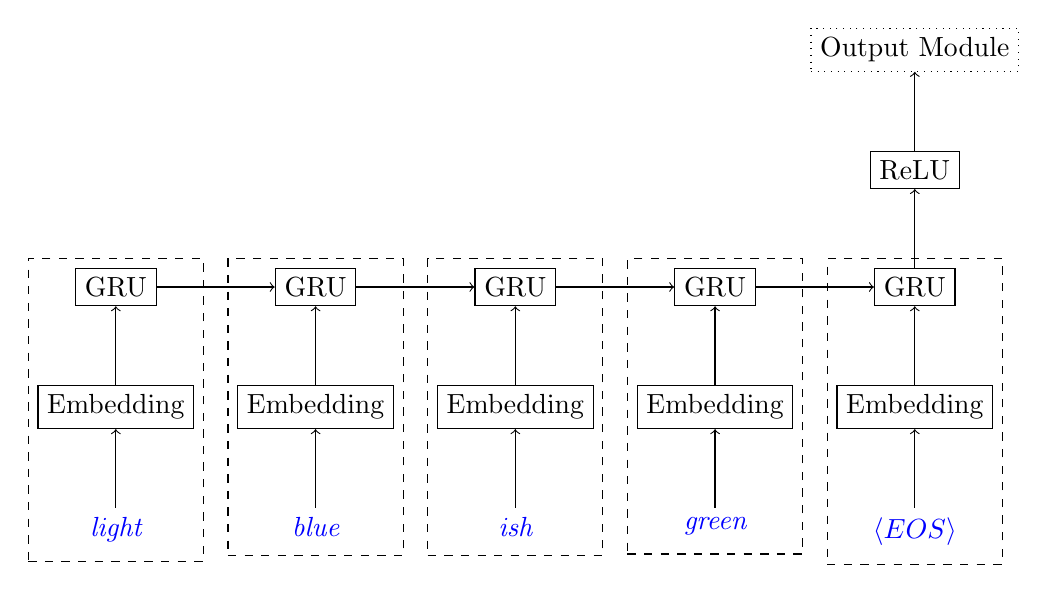
\begin{tikzpicture}
		\node (hiddenoutput)[layer] at (0,0) {ReLU};
		\node (output)[dotted, layer, above=1 of hiddenoutput] {Output Module};
		\draw[->] (hiddenoutput) to (output);
		
		\node (GRU1)[layer, below = of hiddenoutput]{GRU};
		
		\foreach[count=\i from 1] \j in {2,...,5}
		{
			\node (GRU\j)[layer, left = of GRU\i]{GRU};
			\draw[->] (GRU\j) to (GRU\i);
		}
		
		\foreach[count=\i from 1] \word in {$\langle EOS \rangle$, green, ish, blue, light}
		{
			\node (emb\i)[layer, below = of GRU\i]  {Embedding};
			\node (word\i)[word, below = of emb\i]{\word};
			\draw[->] (word\i) to  (emb\i);
			\draw[->] (emb\i) to (GRU\i);
			\node[draw,dashed,fit= (emb\i)  (word\i)  (GRU\i)] {};
		}
		
		
		\draw[->] (GRU1) to (hiddenoutput);
	\end{tikzpicture}

	\caption{The RNN Input module for the example input \natlang{light greenish blue}. Each dashed box represents 1 time-step.}
\end{figure}


A Recurrent Neural Network is a common choice for this kind of task,
due to the variable length of the input.
The general structure of this network, shown in \Cref{fig:rnnmod} is similar to \textcite{2016arXiv160603821M}, or indeed to most other word sequence learning models.
Each word is first transformed to an embedding representation.
This representation is trained with the rest of the network allowing per word information to be efficiently learned.
The embedding is used as the input for a Gated Recurrent Unit (GRU)  \parencite{cho2014properties}.
The output of the last time-step is fed to a Rectified Linear Unit (ReLU)  \parencite{dahl2013reludropout}.


\subsubsection{Sum of Word Embeddings (SOWE)}
Using a simple sum of word embeddings as a layer in a neural network is less typical than an RNN structure.
Though it is well established as a useful representation, and has been used an input to other classifiers such as support vector machines. \pdfcomment{Cite some papers, e.g. mine where this is done.}
Any number of word embeddings can be added to the sum.
However, it has no representation of the order.
The structure we used is shown in \Cref{fig:sowemod}.

\begin{figure}
	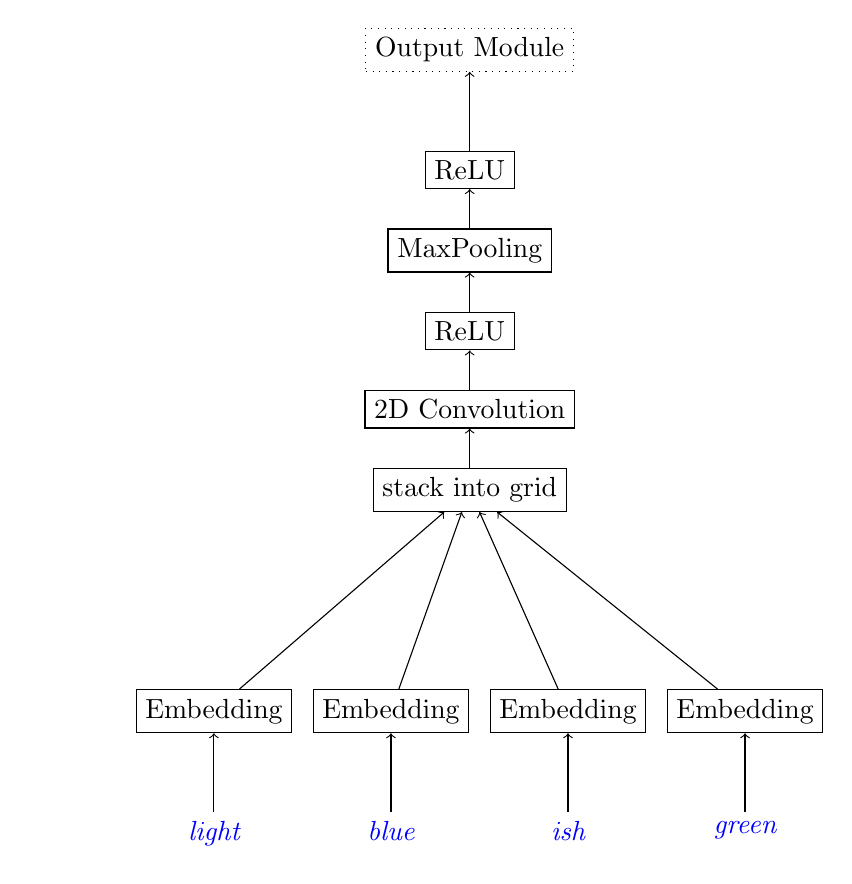
\begin{tikzpicture}

	\node (GRU1)[]{};
	
	\foreach[count=\i from 1] \j in {2,...,5}
	{
		\node (GRU\j)[left = 2 of GRU\i]{};
	}
	
	\node (hstack)[layer, above= of GRU3, xshift=1cm]{stack into grid};
	
	
	\foreach[count=\i from 1] \word in {green, ish, blue, light}
	{
		\node (emb\i)[layer, below = of GRU\i]  {Embedding};
		\node (word\i)[word, below = of emb\i]{\word};
		\draw[->] (word\i) to  (emb\i);
		\draw[->] (emb\i) to (hstack);
	}
	
	\node (conv)[layer, above= 0.5 of hstack]{2D Convolution};
	\node (innerconv)[layer, above= 0.5 of conv]{ReLU};
	\node (pool)[layer, above= 0.5 of innerconv]{MaxPooling};
	\node (hiddenoutput)[layer, above= 0.5 of pool] {ReLU};
	\node (output)[dotted, layer, above=1 of hiddenoutput] {Output Module};
	\draw[->] (hstack) to (conv);
	\draw[->] (conv) to (innerconv);
	\draw[->] (innerconv) to (pool);
	\draw[->] (pool) to (hiddenoutput);
	\draw[->] (hiddenoutput) to (output);
	
%	\draw[->] (hstack) to (hiddenoutput);
%	\draw[->] (hiddenoutput) to (output);
	
	\end{tikzpicture}
	
	\caption{The SOWE input module for the example input \natlang{light greenish blue}}
	\label{fig:sowemod}
\end{figure}


\subsubsection{Convolutional Neural Network(CNN)}

We apply a convulutional neural network to the task by applying 2D convolution over the stacked word embeddings.
\Cref{fig:cnnmod}
We use 64 filters of size between 1 and the length of the longest padded embedding (5).



\begin{figure}
	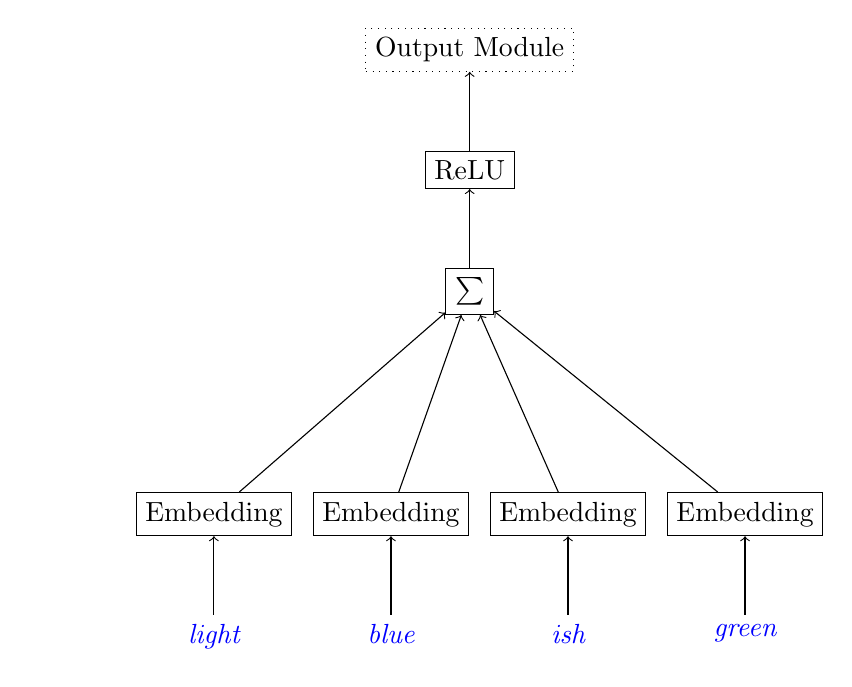
\begin{tikzpicture}
	
	\node (GRU1)[]{};
	
	\foreach[count=\i from 1] \j in {2,...,5}
	{
		\node (GRU\j)[left = 2 of GRU\i]{};
	}
	
	\node (sum)[layer, above= of GRU3, xshift=1cm]{$\sum$};
	
	\foreach[count=\i from 1] \word in {green, ish, blue, light}
	{
		\node (emb\i)[layer, below = of GRU\i]  {Embedding};
		\node (word\i)[word, below = of emb\i]{\word};
		\draw[->] (word\i) to  (emb\i);
		\draw[->] (emb\i) to (sum);
	}
	
	\node (hiddenoutput)[layer, above=of sum] {ReLU};
	\node (output)[dotted, layer, above=1 of hiddenoutput] {Output Module};
	\draw[->] (sum) to (hiddenoutput);
	\draw[->] (hiddenoutput) to (output);
	
	\end{tikzpicture}
	
	\caption{The SOWE input module for the example input \natlang{light greenish blue}}
	\label{fig:sowemod}
\end{figure}



\subsubsection{Non-term based Baseline}
To baseline the performance of our models we propose 
\paragraph{Histogram Baseline (Distribution Estimation, only)}
\paragraph{Mean Squared Error Baseline (Point Estimation, only)}

\subsection{Datasets}


\subsubsection{Full Training and Testing set}
We make use of the  Munroe dataset as prepared by \textcite{mcmahan2015bayesian} from the results of the XKCD color survey.
The XKCD color survey \parencite{Munroe2010XKCDdataset}, collected over 3.4 million observations from over 222,500 respondents.
McMahan and Stone take a subset from Munroe's full survey, by restricting it to the responses from native English speakers, 
and removing very rare color names with less than 100 uses.
This gives a total of 2,176,417 observations and 829 color names. 
They also define a standard test, development and train split.


\subsubsection{Extrapolation Training and Testing Set}
The primary goal in constructing using the term based models is to be able to make predictions for never before seen descriptions of colors.
For example, based on the learned understanding of \texttt{salmon} and of \texttt{bright}, from examples like \texttt{bright green} and \texttt{bright red}, we wish for the systems to make predictions about \texttt{bright salmon}, even though that description never occurs in the training data.
%
To evaluate this generalisation capacity, we define an extrapolation sub-dataset for both testing and training.
This is defined by selecting the rarest 100 color descriptions from the full dataset,
with the restriction that every token in a selected description must still have at least 8 uses in other descriptions in the training set.
The selected examples include multi-token descriptions such as: \texttt{bright yellow green} and also single tokens that occur more commonly as modifiers than as stand-alone descriptions such as \texttt{pale}.

The extrapolation training set is made up of the data from the full training set, excluding those  corresponding the the rare descriptions.
Similar is done for the development set, so as no direct knowledge of the combined terms can leak during early-stopping.
Conversely, the extrapolation test set is made up of only the observations from the full test set that do use those rare descriptions.


By training on the extrapolation training set and testing on the extrapolation test set, we can assess the capacity of the models to make predictions for color descriptions not seen in training.
A similar approach was used in \textcite{DBLP:journals/corr/AtzmonBKGC16}.
We contrast this to the same models when trained on the full training set, but tested on the extrapolation test set, to see how much accuracy was lost.


\subsection{Order Testing set}
It is known that the order of words in a color description to some extent matters.
\natlang{greenish brown} and \natlang{brownish green} are distinct, if similar, colors.
To assess the models on there ability to make predictions when order matters we construct the order testset.
This is a subset of the full test set containing only descriptions with terms that occur in multiple different orders.
There are 76 such descriptions in the full dataset.
Each of which has exactly one alternate ordering.
This is unsurprising as while color descriptions may have more than 2 terms, normally one of the terms is a joining token such as \natlang{ish} or \natlang{-}.



\subsection{Output Modules}
\subsubsection{Distribution Estimation}

For all the distribution estimation systems we investigate here, 
we consider training both on the binned-data, and on the smoothed data (as described in \Cref{sec:kernel-density-based-smoothing}).
Making use of the conditional independence assumption (see \Cref{sec:conditional-independence-assumption}), we output the three discretized distributions.
This is done using 3 softmax output layers.

The output module for distribution estimation 

Contrasting to estimating continuous conditional distributions, 
estimating a discrete conditional distributions is a significantly more studied application of neural networks
-- this is the basic function of any softmax classifier.
To simplify the problem, we therefore transform it to be a discrete distribution estimation task, by discretizing the color-space.
Discretization to a resolution of 64 and 256 bins per channel is considered.


For the case of the machine learning models, the output is produced using softmax layers.


\begin{figure}
	\newcommand{\picwidth}{60pt}
	\begin{tikzpicture}
	
	\node (input)[layer, dotted]{Input Module};
	
	\node(outHue)[layer, above left = of input] {Softmax};
	\node(outSaturation)[layer, above = of input] {Softmax};
	\node(outValue)[layer, above right = of input] {Softmax};
	
	\foreach \p in {Hue, Saturation, Value} 
	{
		\draw[->] (input) to (out\p);
		
		\node(plot\p)[above = of out\p, text width=\picwidth]{
			\includegraphics[width=\picwidth]{netdia/\p}
			\\
			\p
		};
		\draw[->] (out\p) to (plot\p);
	}
	
	\end{tikzpicture}
	
	\caption{The Distribution Output Module \label{fig:distoutmod}}
\end{figure}
	

\subsubsection{Point Estimation}
Our point estimation output model for the neural network is shown in \Cref{fig:pointoutmod}.
The hidden-layer from the top of the input module is feed to an 4 single output neurons.\footnote{Equivalently these 4 single neurons can be expressed as a layer with 4 outputs and 2 different activation functions.}
Two of these are used the sigmoid activation function (range 0:1) to produce the outputs for the saturation and value channels.
The other two use the tanh activation function (range -1:1), they produce the intermediate output that we call $y_{shue}$ and $y_{chue}$ for the sine and cosine of the hue channel respectively.
We use these intermediate values when calculated this loss function as it results in a loss function that is continuous and correctly handles the wrap-around nature of the hue channel.

During training we use the following loss function for each observation $y^\star$, and each corresponding prediction $y$.
\begin{align}
loss &= %
\frac{1}{2} \left(\sin(y^\star_{hue}) - y_{shue} \right)^2  \\
&+ \frac{1}{2} \left(\cos(y^\star_{hue}) - y_{chue} \right)^2  \\
&+ \left(y^\star_{sat} - y_{sat} \right)^2 \\
&+ \left(y^\star_{val} - y_{val} \right)^2 %
\end{align}
This mean of this loss is taken over all observations in each mini-batch during training.





\begin{figure}
	\newcommand{\picwidth}{60pt}
	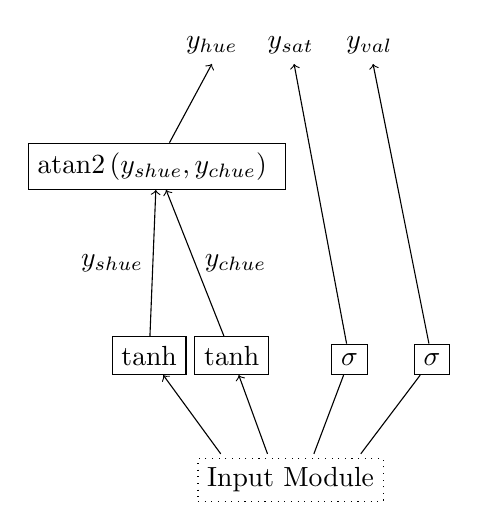
\begin{tikzpicture}
	
	\node (hiddenout)[layer, dotted]{Input Module};
	%\node (hiddenout)[above= 1 of input]{Affine with output width 4};
	%\draw[->](input) to (hiddenout);
	
	\node(outHue)[xshift=-1cm, above = 5 of hiddenout] {$y_{hue}$};
	\node(outSaturation)[above = 5 of hiddenout] {$y_{sat}$};
	\node(outValue)[xshift=1cm, above = 5 of hiddenout] {$y_{val}$};
	
	\node(Z)[above=-0.2cm of hiddenout.north]{};
	\node(Z2)[left=0cm of Z]{};%{$z_2$};
	\node(Z1)[left=0.3cm of Z2]{};%{$z_1$};
	\node(Z3)[right=0cm of Z]{};%{$z_3$};
	\node(Z4)[right=0.3cm of Z3]{};%{$z_4$};
	
	
	\node(s3)[layer, above=1 of Z3, xshift=0.5cm]{$\sigma$};
	\node(s4)[layer, above=1 of Z4, xshift=1cm]{$\sigma$};
	\draw[->](Z3) to (s3) to (outSaturation);
	\draw[->](Z4) to (s4) to (outValue);
	
	
	\node(AngHue)[layer, below = 1 of outHue, xshift=-0.7cm]{$ \mathrm{atan2} \left(y_{shue}, y_{chue} \right) $ };
	\draw[->](AngHue) to (outHue.south);
	
	\node(s1)[layer, above=1 of Z1, xshift=-1cm]{$\tanh$};
	\node(s2)[layer, above=1 of Z2, xshift=-0.5cm]{$\tanh$};
	\draw[->](Z1) to (s1);
	\draw[->](s1) to node[left]{$y_{shue}$} (AngHue);
	\draw[->](Z2) to (s2);
	\draw[->](s2) to node[right]{$y_{chue}$}  (AngHue);
	
	
	
	
	
	\end{tikzpicture}
	
	\caption{The Point Estimate Output Module.
		Here $\mathrm{atan2}$ is the quadrant preserving arctangent, outputting as a regularized angle (as per in all evaluations).
		 \label{fig:pointoutmod}}
\end{figure}






\clearpage
\bibliography{master}

\clearpage
\appendix
\documentclass[11pt,a4paper]{article}
\usepackage{times}
%\usepackage[author={Lyndon}]{pdfcomment}

\usepackage{booktabs}
\usepackage{pgfplotstable}
\pgfplotsset{compat=1.14}


\usepackage{amssymb}
\usepackage{amsmath}
\usepackage{mathtools}
\DeclareMathOperator*{\argmin}{arg\,min}
\DeclareMathOperator*{\argmax}{arg\,max}


\usepackage{cleveref}


\title{Learning of Colors from Color Names: \\ Distribution and Point Estimation\\Supplementary Materials}
\author{}
\date{}

\begin{document}
\maketitle

\section{On the Conditional Independence of Color Channels given a Color Name}\label{sec:corrind}

As discussed in the main text, we conducted a superficial investigation into the truth of our assumption that given a color name, the distributions of the hue, value and saturation are statistically independent.

We note that this investigation is, by no means, conclusive though it is suggestive.
The investigation focusses around the use of Spearman's rank correlation.
This correlation measures the monotonicity of the relationship between the random variables.
A key limitation is that the relationship may exist but be non-monotonic.
This is almost certainly true for any relationship involving channels, such as hue, which wrap around.
In the case of such relationships Spearman's correlation will underestimate the true strength of the relationship.
Thus, this test is of limited use in proving the conditional independence.
However, it is a quick test to perform and does suggest that the conditional independence assumption may not be so incorrect as one might assume.


For the Monroe Color Dataset training data  given by $V \subset \mathbb{R}^{3}\times T$, where $\mathbb{R}^{3}$ is the value in the color-space under consideration, and $T$ is the natural language space.
The subset of the training data for the description $t \in T$ is given by
$V_{|t}=\{(\tilde{v}_i,\,t_i) \in V \: \mid \: t_{i}=t\}$.
Further let $T_V = \{t_i \: \mid \: (\tilde{v},t_i)\in V$ be the set of color names used in the training set.
Let $V_{\alpha|t}$ be the $\alpha$ channel component of $V_{|t}$, i.e. $V_{\alpha|t} = \left\lbrace v_\alpha \mid ((v_1,v_2,v_3), t) \in V_{|t} \right\rbrace$.

The set of absolute Spearman's rank correlations between channels $a$ and $b$ for each color name is given by
$S_{ab}=\left\lbrace \left|\rho(V_{a|t},V_{b|t})\,\right|\,t\in T_{V}\right\rbrace$.
\newpage

We consider the third quartile of that correlation as the indicative statistic in \Cref{tbl:colorcor}.
That is to say for 75\% of all color names, for the given color-space, the correlation is less than this value.



Of the 16 color-spaces considered, it can be seen that the HSV exhibits the strongest signs of conditional independence -- under this (mildly flawed) metric.
More properly put, it exhibits the weakest signs of non-independence.
This includes being significantly less correlated than other spaces featuring circular channels such as HSL and HSI.

Our overall work makes the conditional independence assumption, much like n-gram language models making Markov assumption.
The success of the main work indicates that the assumption does not cause substantial issues.


\pgfkeys{/pgf/number format/.cd, fixed relative, precision=4}
\pgfplotstableset{corstyle/.append style={%
		col sep=tab,
		header=has colnames,
		columns/Color Space/.style={reset styles, string type, column name=Color-Space},
		ignore chars={"},
		every head row/.style={before row=\toprule,	after row=\midrule}
	}%
}

\begin{table}
	\centering
%	\resizebox{\columnwidth}{!}{
		\pgfplotstabletypeset[corstyle]{results/colorcor.tsv}
%	}
	\caption{\label{tbl:colorcor} The third quartile for the pairwise Spearman's correlation of the color channels given the color name.}
	
\end{table}

\section{KDE based smoothing of Training Data}\label{sec:smoothed-results}

It can be seen that smoothing has very little effect on the performance of any of the neural network based distribution estimation models.
All 3 term based models (SOWE, CNN, RNN) all perform very similarly whether or not the training data is smoothed.
This is seen consistently in all the distribution estimation tasks.
Contrast \Cref{tbl:distfull-smoothed,tbl:distord-smoothed,tbl:distextrapo-smoothed}
to the tables for the unsmoothed results
\Cref{tbl:distfull,tbl:distord,tbl:distextrapo}.

If however, smoothing is not applied to the Operational Upper Bound, it works far worse.
In  \Cref{tbl:distfull-smoothed,tbl:distord-smoothed,tbl:distextrapo-smoothed} the Direct result refers to using the training histograms almost directly, without any smoothing or term-based input processing.
This is the same as the Operation Upper Bound, minus the KDE.
It works very poorly (by comparison).
This is because the bins values are largely independent: a very high probability in one bin does not affect the probability of the adjacent bin -- which by chance of sampling my be lower than the trust distribution would have it.

This is particularly notable in the case of the direct, full training set result on the unseen combinations task reported  in \Cref{tbl:distextrapo-smoothed}. As these were some of the rarest terms in the training set, several did not coincide with any bins for observations in testing set.
This is because without smoothing it results in estimating the probability based on bins unfilled by any observation.
We do cap that empty bin probability at $\epsilon_{64} \approxeq 2\times 10^{-16}$ to prevent undefined perplexity.
(We found capping the lower probability for bins like this to be far more effective than add-on smoothing).

Conversely, on this dataset the neural network models do quiet well, with or without smoothing.
As the network can effectively learn the smoothness, not just from the observations of one color but from all of the observations.
It learns that increasing the value of one bin should increase adjacent ones.
As such it does not need the smoothing applied to the training data.

\pgfkeys{
	/pgf/number format/.cd, fixed, precision=3, fixed zerofill=true
}

\pgfplotstableset{
	col sep=comma,
	header=has colnames,
	column type={c},
	ignore chars={"},
	string replace={Direct}{\emph{Direct}},
	clear infinite,
	empty cells with={--},
	every head row/.style={before row=\toprule,	after row=\midrule},
	columns/method/.style={reset styles, string type, column name=Method},
	%
	boldcell/.style = {
		postproc cell content/.append style={
			@cell content/.add={\mathversion{tabularbold}}{}
		}
	},
	%
	greycell/.style = {
		postproc cell content/.append style={
			@cell content/.add={\color{gray}}{}
		}		
	}
}
\pgfplotstableset{distresults/.append style={%
		columns={method, perpstd},
		columns/perp/.style={column name=$PP$},
		create on use/perpstd/.style={
			create col/expr={\thisrow{perp}/(256*256*256)},
		},
		columns/perpstd/.style={column name=$\frac{PP}{256^3}$},
		%
		every row 0 column 1/.style={greycell}
	},%
	%%%%%%%%%%%%%%%%%%%%%%%%%%%%%%%%%%%%%%%%%%%%%%%%
	extrapodistresults/.append style={
		every row 0 column 1/.style={greycell},
		every row 0 column 2/.style={greycell},
		%
		columns={method, nxperpstd, xperpstd},
		columns/nxperpstd/.style={column name={\shortstack{\small Full\\Training Set\\$\frac{PP}{256^3}$}}},
		columns/xperpstd/.style={column name={\shortstack{\small Restricted\\Training Set\\$\frac{PP}{256^3}$}}},
		%		
		create on use/xperpstd/.style={
			create col/expr={\thisrow{extrapolatingperp}/(256*256*256)},
		},
		create on use/nxperpstd/.style={
			create col/expr={\thisrow{nonextrapolatingperp}/(256*256*256)},
		},
	}
}

\begin{table}
	%	\resizebox{\columnwidth}{!}{
	\pgfplotstabletypeset[distresults,
	every row 1 column 1/.style={greycell},
	]{results/smoothed/res_dist_full.csv}
	%	}
	\caption{\label{tbl:distfull-smoothed}  The results for the \textbf{full distribution estimation task} using smoothed training data. Lower perplexity (PP) is better. This corresponds to the main results \Cref{tbl:distfull}.}
\end{table}




\begin{table}
	%	\resizebox{\columnwidth}{!}{
	\pgfplotstabletypeset[distresults,
	every row 1 column 1/.style={greycell},
	]{results/smoothed/res_dist_ord.csv}
	%	}
	\caption{\label{tbl:distord-smoothed}  The results for the \textbf{order distribution estimation task} using smoothed training data. Lower perplexity (PP) is better. This is a subset of the full test set containing only tests where the order of the words matters. This corresponds to the main results \Cref{tbl:distord}.}
\end{table}


\begin{table}
	%	\resizebox{\columnwidth}{!}{
	\pgfplotstabletypeset[extrapodistresults,
	every row 1 column 1/.style={greycell},
	every row 1 column 2/.style={greycell},
	]{results/smoothed/res_dist_extrapo.csv}
	%	}
	\caption{\label{tbl:distextrapo-smoothed}  The results for the \textbf{unseen combinations distribution estimation task} using smoothed training data. Lower perplexity (PP) is better. This uses the extrapolation subset of the full test set. In the extrapolating results certain rare word combinations were removed from the training and development sets. In the non-extrapolating results the full training and development stet was used. This corresponds to the main results \Cref{tbl:distextrapo}.}
\end{table}
%%%%%%%%%%%%%%%%%%%%%%%%%%%%%%%%%%%%%%%%%%%%%%%%%%%%%%%%%%%%%%%%%%%%%%%%%%%%%%%%%%%%%%%%%%%%%%%%%%%%%%%%%%%
%
%\pgfplotstableset{pointresults/.append style={%
%		columns={method,mse},
%		columns/mse/.style={column name={$MSE$}},
%		%
%		every row 0 column 1/.style={greycell},
%		every row 4 column 1/.style={greycell},
%	},%
%	extrapopointresults/.append style={
%		columns={method, nonextrapolatingmse, extrapolatingmse},
%		columns/nonextrapolatingmse/.style={column name=\shortstack{\small Full\\Training Set\\$MSE$}},
%		columns/extrapolatingmse/.style={column name=\shortstack{\small Restricted\\Training Set\\$MSE$}},
%		%		
%		every row 0 column 1/.style={greycell},
%		every row 4 column 1/.style={greycell},
%		every row 0 column 2/.style={greycell},
%		every row 4 column 2/.style={greycell},
%	},
%}
%
%
%\begin{table}
%	%	\resizebox{\columnwidth}{!}{
%	\pgfplotstabletypeset[pointresults,
%	every row 2 column 1/.style={boldcell},
%	every row 1 column 1/.style={boldcell}
%	]{results/smoothed/res_point_comb_full.csv}
%	%	}
%	\caption{\label{tbl:pointfull-smoothed}  The results for the \textbf{full point estimation task} using smoothed training data. Lower mean squared error (MSE) is better. This corresponds to the main results \Cref{tbl:pointfull}.}
%\end{table}
%
%
%
%\begin{table}
%	%	\resizebox{\columnwidth}{!}{
%	\pgfplotstabletypeset[pointresults,
%	every row 1 column 1/.style={boldcell},
%	every row 2 column 1/.style={boldcell},
%	%3
%	%4
%	%
%	every row 5 column 1/.style={boldcell},
%	every row 6 column 1/.style={boldcell}
%	]{results/smoothed/res_point_comb_ord.csv}
%	%	}
%	\caption{\label{tbl:pointord-smoothed}  The results for the \textbf{order point estimation task} using smoothed training data. Lower mean squared error (MSE) is better. This is a subset of the full test set containing only tests where the order of the words matters. This corresponds to the main results \Cref{tbl:pointord}.}
%\end{table}
%
%
%\begin{table}
%	%	\resizebox{\columnwidth}{!}{
%	\pgfplotstabletypeset[extrapopointresults,
%	every row 1 column 1/.style={boldcell},
%	every row 2 column 2/.style={boldcell},
%	]{results/smoothed/res_point_comb_extrapo.csv}
%	%	}
%	\caption{\label{tbl:pointextrapo-smoothed}  The results for the \textbf{unseen combinations point estimation task} using smoothed training data. Lower mean squared error (MSE) is better. This uses the extrapolation subset of the full test set. In the extrapolating results certain rare word combinations were removed from the training and development sets. In the non-extrapolating results the full training and development stet was used. This corresponds to the main results \Cref{tbl:pointextrapo}.}
%\end{table}


\end{document}

\end{document}
